\documentclass{../style/sig-alternate}

\usepackage{here}
\usepackage{url}

%----------- マクロ ----------
%数式番号を節毎に分けてリセットする
\def\theequation{\thesection.\arabic{equation}}
  \makeatletter
  \@addtoreset{equation}{section}
  \makeatother
%図番号を節毎に分けてリセットする
\makeatletter
 \renewcommand{\thefigure}{%
   \thesection.\arabic{figure}}
  \@addtoreset{figure}{section}
\makeatother
%表番号を節毎に分けてリセットする
\makeatletter
 \renewcommand{\thetable}{%
   \thesection.\arabic{table}}
  \@addtoreset{table}{section}
\makeatother

\makeatletter
 \let\@copyrightspace\relax
 \makeatother

\begin{document}

\title{SLSTC at the NTCIR-12 STC Task}

\numberofauthors{5}
\author{
% You can go ahead and credit any number of authors here,
% e.g. one 'row of three' or two rows (consisting of one row of three
% and a second row of one, two or three).
%
% The command \alignauthor (no curly braces needed) should
% precede each author name, affiliation/snail-mail address and
% e-mail address. Additionally, tag each line of
% affiliation/address with \affaddr, and tag the
% e-mail address with \email.
%
% 1st. author
\alignauthor
Hiroto Denawa\\
       \affaddr{Waseda University}\\
       \email{hi\_denawa@fuji.waseda.jp}
% 2nd. author
\alignauthor
Tomoaki Sano\\
       \affaddr{Waseda University}\\
       \email{tonosamoaki@asagi.waseda.jp}
\and  % use '\and' if you need 'another row' of author names
% 3rd. author
\alignauthor
Yuta Kadotami\\
       \affaddr{Waseda University}\\
       \email{kdtm-783640@ruri.waseda.jp}
% 4th. author
\alignauthor
Sosuke Kato\\
       \affaddr{Waseda University}\\
       \email{sow@suou.waseda.jp}
%\and  % use '\and' if you need 'another row' of author names
% 5th. author
\alignauthor
Tetsuya Sakai\\
       \affaddr{Waseda University}\\
       \email{tetsuyasakai@acm.org}
}

\maketitle

\begin{abstract}
The SLSTC team participated in the NTCIR-12 Short Text Conversation
(STC) task.
This report describes our approach to solving the STC problem and discusses the
ocial results.
\end{abstract}

\section*{Team Name}
SLSTC

\section*{Subtasks}
Japanese subtask

\keywords{STC; HNN; Word2Vec; PageRank; word co-occurrence network}

\section{Introduction}

SLSTC (The Sakai Laboratory, Waseda University) participated in the
Japanese subtask of the STC task.
This paper briefly describes our approaches,
and reports on the official results.

Table \ref{tab:run_list}  shows the list of runs that we submitted to the STC Japanese subtask.
In Section~\ref{sec:methods}, we describe the algorithms we employed
to generate these runs.
In Section~\ref{sec:results}, we discuss the official results of our runs.
Finally, in Section~\ref{sec:conclusions}, we conclude this paper
and lists up future work items.

\begin{table}[h!]
  \centering
  \caption{the list of runs}
  \label{tab:run_list}
  \begin{tabular}{|c|} \hline
     run name \\ \hline
     SLSTC-J-R1 \\ \hline
     SLSTC-J-R2 \\ \hline
     SLSTC-J-R3 \\ \hline
  \end{tabular}
\end{table}

\section{Methods}
\label{sec:methods}

\subsection{SLSTC-J-R1}

This run was generated by the second author (Tomoaki Sano), as his bachelor's thesis project.

First, Word2Vec \footnote{\url{http://code.google.com/p/word2vec/}} is utilised 
to generate a distributed representation for every term in a tweet. Japanese Wikipedia and Nicopedia (Niconico Daihyakka) were used as the corpora. Thus every term is represented as a word vector. Second, a tf-idf weight for each term in a tweet and the word vectors are weighted accordingly. The tweet is then represented as the sum of the weighted word vectors. Third, a three-layered neural network is used for generating a reply from a post. Finally, the STC repository is searched and 
the top five replies that are most similar to the output from the neural network are 
included in the run file.

\subsection{SLSTC-J-R2 and SLSTC-J-R3}
These two runs were generated by the first, third, and the fourth authors as a collaboration project.
Our method is based on a word co-occurrence network, and it consists of three parts:
network construction, subnetwork extraction, and ranked output generation.

\subsubsection{Network Construction}
In this part, we make a word co-occurrence network from post-reply tweet pairs.
As the datset, 427200 post-reply tweet pairs are provided from NTCIR.
First, we perform morphological analysis on the tweet pairs using MeCab\cite{mecab}. Then we extract pair of sets of noun words from each pair as \((W_{p}, W_{r})\). Wp or Wr contains a ordered word set which means faster word appear faster in the original tweet. And set \(V\) as an union of all pairs.

\begin{enumerate}
    \item \(W_{p} = (w_{p1}, w_{p2}, ... w_{pi} ... w_{pn}) \)
    \item \(W_{r} = (w_{r1}, w_{r2}, ... w_{ri} ... w_{rn}) \)
    \item \(P = \{W | W \in \bigcup W_{p} \wedge W \in \bigcup W_{r}\}\)
    \item \(V = \{w | w \in W \wedge W \in P\} \)
\end{enumerate}

Using V as nodes, we make a directed graph. We make a path from the first word in some tweet to the next word in the tweet and from each word in \( W_{p} \) to all words in \(W_{r} \).

\begin{eqnarray}
\begin{split}
E = &\{(w_{1}, w_{2}) | w_{1}\in W_{p} \lor w_{2}\in W_{r}\}\\
&\cup \{(w_{pi}, w_{p(i+1)}) | 0 < i < n-1\}\\
&\cup \{(w_{ri}, w_{r(i+1)}) | 0 < i < n-1\}
\end{split}
\end{eqnarray}


At last a word co-occurrence network G is defined like below:

\begin{eqnarray}
G := (V,E)
\end{eqnarray}

This word network shows what word likely appear next to some word. In other words, it shows that how wrods close to each other. So, it represents word distribution which contains topic distribution.

\subsubsection{Subnetwork Extraction}
Test tweet data is same as the data used in RUN1. As well as previous part, we extract set of noun words from each test tweet as \(W_{t} = (w_{t1}, w_{t2}, ... w_{ti} ... w_{tn})\).
In this part, we extract subnetwork $G'_{i}$ which contains \(w_{ti}\) from $G$.
If wti exists in V, pick up all nodes which is next to wti.

\begin{eqnarray}V'_{i} = w_{ti} \cup \{w_{e} |  (w_{ti}, w_{e}) \in E\}\end{eqnarray}
\begin{eqnarray}E'_{i} = \{(w_{ti}, w_{e}) | (w_{ti}, w_{e}) \in E\} \end{eqnarray}

Finaly, we get a subnetwork G' like below:

\begin{eqnarray}G'_{i} = (V'_{i}, E'_{i})\end{eqnarray}

\(G' = \bigcup G'_{i}\) represents potential topics of expected replies.

\subsubsection{Ranked Output Generation}
In this part, we get results for each $W_{t}$ using subnetworks we get previous part. We add score to each possible reply using the score like tf-idf and PageRank\cite{PageRank}.

First, we calculate PageRank for each word in $W_{t}$. With $E(w_{k})$, which is the number of edges that has $w_{k}$ as the start node, a PageRank is calculated. And $d$ is some parameter set $0.9$ in our experiment.

\begin{eqnarray}PR(w_{ti}) = \frac{(1-d)}{N} + \sum_{w_{k}\in V'_{i}} d(\frac{PR(w_{k})}{E(w_{k})})\end{eqnarray}

Then, we calculate final score with tf-idf like score. $P'$ is a set of tweets which concludes $w_{ti}$. 

\begin{eqnarray}P'_{ij} = \{W_{j} | W_{j} \in P \wedge w_{ti} \in W_{j}\}\end{eqnarray}

And, we define $df$ as the number of tweets in $P'$, $N$ as the number of tweets in $P$, $l$ as the number of word in $W_{i}$, and tc as how many $w_{ti}$ appear in $W_{i}$.

\begin{enumerate}
    \item $df_{i} = n(P'_{ij})$
    \item $N = n(P)$
    \item $idf = \log_{10} \frac{N}{df} + 1$
    \item $l_{i} = n(W_{j})$
    \item $tc_{i} = n(\{w | w = w_{ti} \wedge w \in W_{j}\})$
\end{enumerate}

Finaly, the score is caculated like below:

\begin{eqnarray}Score(W_{j}) = \sum_{i} \frac{l-tc+1}{l} idf PR(w_{ti})\end{eqnarray}

Following this score, our system return the rank list of $W_{j}$ against each test data $W_{t}$.

\subsubsection{Two types of system}

  We analyzed result of this run. We considered that continuous ``w'' was noise. So, we remove morpheme include continuous ``w''.
  Our submition of Run2 is type of not removed ``w'', and Run3 is type of removed ``w''.



\section{Official Results and Discussions}
\label{sec:results}
Table \ref{tab:results} shows the results of our systems, the maximam score of the other systems and the minimum score of the other systems. 
``ACX-Y'' means that X indicates what score is regarded as true output and Y indicates the range of the acceptable rank. For example, ``AC12-1'' means that the outputs scored 1 or 2 and having top rank is evaluated.

From the results, our systems seem not to work. To know what kind of trouble occures in our system, we analyzed details of the results.


Figure \ref{fig:run2} and fiqure \ref{fig:run3} show what tweet appeared frequently as a possible reply. This table indicates our system provide a nealy same set of tweets as possible replies. So, our results does not relate to inputs strongly. Something is wrong with our scoring algorithms. For, we analyzed the structure of subnetworks and its PageRank, TF and IDF.


Table \ref{tab:subnetwork1} and table \ref{tab:subnetwork2} show what words are enabled as a input and what words appear in a subnetwork for each input.
The accuracy of both outputs are relatively low: 0.04 for the former one, 0.16 for the latter one in ``AC12-5''. But, the words in the former result seem to be connected to inputs. For example, in input words, \mbox{``各駅停車''} and \mbox{``神戸三宮''} are words related to transpotation facility. And, in the subnetwork, \mbox{``バスターミナル''} is also a word related to transpotation facility. Why is accuracy low? We think this is caused by too many words in each subnetwork. Too many words in a subnetwork makes too low PageRank for each word. That means all scores of the output tweets reflect TF and IDF directly.
On the other hands, the words in the latter result seem not to be connected to inputs. To begin with, the words \mbox{``さんが''}, \mbox{``プラス''}, \mbox{``して''} seem to indicate no topics. The system failed to perform morphological analysis appropriately.


So, in both cases, the results of our system does not reflect input topics. Instead, the data only about the frequency of words effects the results. So, our system outputs almost the same set of tweets.

\begin{table}[h!]
  \centering
  \caption{The results}
  \label{tab:results}
  \begin{tabular}{|c|c|c|c|c|} \hline
      & AC2-1 & AC2-5 & AC12-1 & AC12-5 \\ \hline
     SLSTC-J-R1 & 0.0381 & 0.0364 & 0.1644 & 0.1650 \\ \hline
      SLSTC-J-R2 & 0.0782 & 0.0332 & 0.3416 & 0.1795\\ \hline
      SLSTC-J-R3 & 0.0054 & 0.0032 & 0.0391 & 0.0196\\ \hline
      MAX & 0.4574 & 0.3583 & 0.7817 & 0.7050\\ \hline
      MIN & 0.0054 & 0.0032 & 0.0391 & 0.0196\\ \hline
  \end{tabular}
\end{table}

\begin{figure}[t!]
\begin{center}
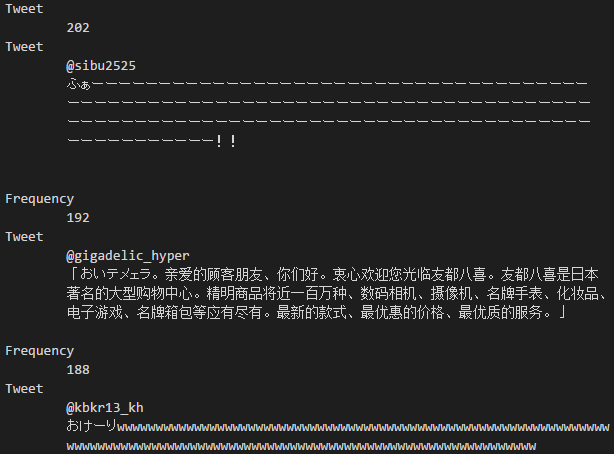
\includegraphics[width=120mm,bb=0 0 816 579]{../img/run2.png}
\caption{Top 3 tweets appearing in the results of run 2}
\label{fig:run2}
\end{center}
\end{figure}

\begin{figure}[t!]
\begin{center}
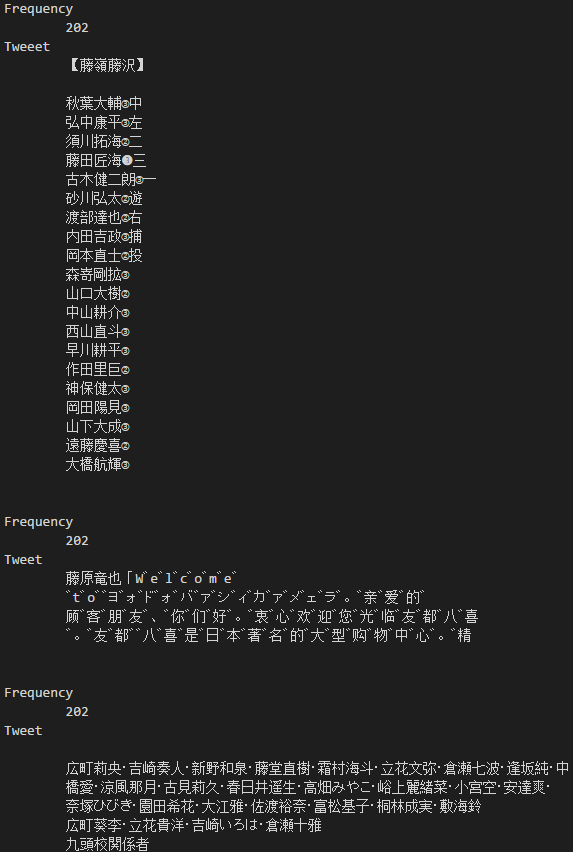
\includegraphics[width=120mm,bb=0 0 816 579]{../img/run3.png}
\caption{Top 3 tweets appearing in the results of run 3}
\label{fig:run3}
\end{center}
\end{figure}


\begin{table*}
    \begin{center}
    \caption{top 3 PageRank * IDF score words in subnetwork for some input}
    \label{tab:subnetwork1}
    \begin{tabular}{|p{20em}|p{5em}|p{5em}|c|c|c|} \hline
    input & noun & word & PageRank & IDF & PageRank*IDF\\ \hline
    & & PCゲーム & 2.96e-5 & 4.75 & 0.000141\\ \cline{3-6}
    ゆうくりっどさんが言いたいことにプラスして言及してくれてた & さんが, プラス, して & トレシュー & 2.40e-5 & 5.23 & 0.000125\\ \cline{3-6}
    & & 女川 & 2.37e-5 & 5.23 & 0.000124\\ \hline
    \end{tabular}
    \end{center}
\end{table*}


\begin{table*}
    \begin{center}
    \caption{top 3 PageRank * IDF score words in subnetwork for some input}
    \label{tab:subnetwork2}
    \begin{tabular}{|p{20em}|p{5em}|p{5em}|c|c|c|} \hline
    input & noun & word & PageRank & IDF & PageRank*IDF\\ \hline
    & & ゃんいってらっしゃいだよっ & 2.08e-5 & 5.23 & 0.000109\\ \cline{3-6}
    【自動】\newline お待たせしました。\newline 7号線、各駅停車、神戸三宮行き\newline ただいま発車します。 & 自動, 7号, 各駅停車, 神戸三宮 & バスターミナル & 1.87e-5 & 5.23 & 9.75e-5\\ \cline{3-6}
    & & PCゲーム & 1.87e-05 & 4.75 & 8.87e-5\\ \hline
    \end{tabular}
    \end{center}
\end{table*}

\section{Conclusions and Future Work}
\label{sec:conclusions}
We made systems with Neural Network or word co-occurrence network. In this task, we did not get good results but few conclusions like below.

For the system using a word co-occurrence network, we need to improve accuracy of morphological analysis and the mothod for generating subnetwork.
In particular, for performing morphological analysis, we will try to improve the accuracy of dictionary or to handle newer or unknown words appropriately. And, for decreasing tne number of edges of nodes in each subnetwork, we will try to define something weight of the edge or to set strict condition on generating edges in a word co-occurrence network.

\begin{thebibliography}{99}

%\bibitem{sakai} Sakai, T., Shang, L., Lu, Z. and Li, H.: Topic Set Size Design with the Evaluation Measures for Short Text Conversation, AIRS 2015, LNCS 9460, pp.1-13, 2015.
\bibitem{word2vec} Google Word2Vec, https://code.google.com/p/word2vec/
\bibitem{mecab} MeCab, http://taku910.github.io/mecab/
\bibitem{bahman} Bahman Kermanshahi, Construction and Application of Neural Network,Shokodo
\bibitem{PageRank} Sergey Brin, Rajeev Motwani, and Terry Winograd. What can you do with a
web in your pocket. Data Engineering Bulletin, Vol. 21, pp. 37-47, 1998.

\end{thebibliography}


\end{document}
